\section{Masalah Keamanan dalam Komunikasi}
\label{sec:masalah-keamanan}

Ketika menggunakan saluran komunikasi publik, muncul beberapa risiko keamanan yang
harus diatasi. Risiko-risiko itu biasanya diringkas menjadi empat pertanyaan.
Menariknya, keempatnya berbentuk pertanyaan yang wajar diajukan oleh pihak-pihak
yang berkomunikasi, bukan pertanyaan yang diajukan seorang ahli matematika. Hal ini
penting untuk disadari: kriptografi tumbuh dari kebutuhan praktis, dan barulah
kemudian dirumuskan secara matematis.

\subsection{Kerahasiaan (Confidentiality)}

Bagaimana Alice memastikan pesan-pesannya tidak dapat dibaca oleh penyadap
(\textit{eavesdropper}) yang menguping komunikasinya dengan Bob? Inilah yang
disebut masalah kerahasiaan.

Perhatikan bahwa masalah ini tidak menuntut pesannya tersembunyi dari pandangan
penyadap, melainkan tersembunyi maknanya. Penyadap boleh saja melihat seluruh
deretan bit yang melintas; yang harus dijaga adalah agar deretan bit itu tidak
bermakna apa pun baginya. Inilah sebabnya enkripsi bekerja dengan mengubah
representasi pesan, bukan dengan menyembunyikan keberadaan pesan. Sebuah pesan
militer yang berbunyi ``serang fajar besok'' dapat berubah menjadi rentetan huruf
tanpa makna; panjangnya bahkan boleh sama, tetapi kandungan informasinya tertutup.
Gambar \ref{fig:penyadapan-confidentiality} menggambarkan situasi ini.

Perlu ditegaskan bahwa kerahasiaan yang sesungguhnya tidak boleh bergantung pada
kerahasiaan algoritmanya. Prinsip ini dirumuskan oleh Auguste Kerckhoffs pada abad
ke-19 dan diulang oleh Claude Shannon dalam bentuk yang lebih tajam: musuh mengenal
sepenuhnya sistem yang dipakai, dan satu-satunya rahasia adalah kuncinya
(\citealp{schneier1996}). Konsekuensi praktisnya besar --- algoritma boleh (bahkan
harus) diperiksa publik, dan setiap penambalan keamanan cukup dilakukan pada kunci.

\subsection{Otentikasi (Authentication)}

Bagaimana cara Bob memastikan bahwa pesan tersebut benar-benar berasal dari Alice
dan bukan dari pihak ketiga (misalnya Carol) yang menyamar menjadi Alice?

Masalah ini terasa sepele sampai kita menyadari bahwa pada saluran publik tidak ada
yang dapat memastikan identitas secara otomatis. Sebuah surel dapat dikirim dengan
alamat pengirim palsu; sebuah panggilan telepon dapat berasal dari nomor yang
dipalsukan; sebuah paket data dapat memuat alamat sumber yang tidak benar. Bahkan
bila kerahasiaan sudah dijamin sekalipun, penyerang tetap dapat mengirimkan pesan
terenkripsi dengan kunci yang benar sambil mengaku sebagai orang lain. Karena itu
kerahasiaan dan otentikasi adalah dua masalah yang berbeda, meskipun keduanya sama
sekali tidak dapat diselesaikan tanpa kriptografi.

\subsection{Integritas Data (Data Integrity)}

Bagaimana cara Bob memastikan bahwa pesan dari Alice masih utuh, asli, dan tidak
dimanipulasi selama proses pengiriman?

Bayangkan sebuah stasiun cuaca mengirimkan pembacaan suhu $33^{\circ}$C, lalu pihak
yang tidak berwenang mengubahnya menjadi $32^{\circ}$C selama perjalanan. Perubahan
satu angka pada pesan berukuran kecil sekalipun dapat berakibat besar: sebuah
keputusan penerbangan, sebuah transaksi keuangan, atau sebuah diagnosis medis.
Gambar yang hampir sama tetapi berbeda pada satu detail adalah contoh klasik
pelanggaran integritas. Perhatikan bahwa pada contoh ini kerahasiaan tidak
dilanggar --- nilai suhunya memang boleh diketahui siapa saja --- tetapi
integritasnya rusak. Inilah alasan mengapa layanan integritas harus dipandang
sebagai masalah tersendiri.

\subsection{Nir-penyangkalan (Non-repudiation)}

Bagaimana Bob dapat membuktikan bahwa Alice benar-benar mengirim pesan tersebut jika
di kemudian hari Alice menyangkal telah mengirimkannya?

Contoh yang paling gamblang adalah perintah transfer dana. Bila Alice memerintahkan
bank memindahkan sejumlah uang, lalu kemudian ia menyatakan tidak pernah
memerintahkan hal itu, bank harus dapat membuktikan sebaliknya di hadapan pihak
ketiga, misalnya pengadilan. Perhatikan bahwa jawaban seperti ``saya menerima
pesannya'' tidak cukup, sebab Bob dapat saja mengarang pesan itu sendiri. Yang
dibutuhkan adalah bukti yang tidak dapat disangkal oleh Alice, dan bukti semacam itu
harus dapat diperiksa oleh pihak yang netral. Persoalan inilah yang nantinya
melahirkan tanda tangan digital, yang dibahas pada Bab~\ref{chap:tanda-tangan-pki}.

\begin{figure}[htbp]
    \centering
    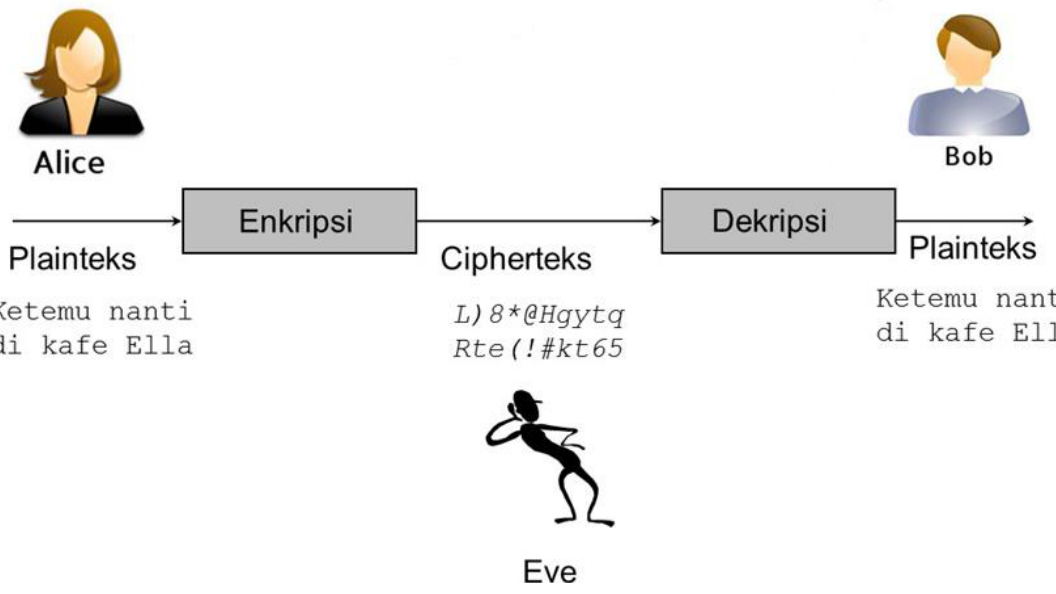
\includegraphics[width=0.78\linewidth, height=0.7\textheight, keepaspectratio]{figures/penyadapan-confidentiality.png}
    \caption{Penyadap hanya dapat melihat cipherteks ketika Alice mengirim pesan terenkripsi kepada Bob, sehingga isi pesan tetap terjaga kerahasiaannya}
    \label{fig:penyadapan-confidentiality}
    \sumber{Munir, \textit{IF4020 Kriptografi}, ITB.}
\end{figure}

Keempat pertanyaan di atas --- kerahasiaan, otentikasi, integritas, dan
nir-penyangkalan --- akan muncul berulang kali sepanjang buku ini. Setiap algoritma
yang dibahas pada bab-bab berikutnya pada akhirnya dapat dinilai dari jawabannya
terhadap salah satu di antara keempatnya. Tabel~\ref{tab:empat-masalah} merangkum
keempatnya beserta contoh pelanggaran yang khas.

\begin{table}[htbp]
    \centering
    \caption{Empat masalah keamanan komunikasi beserta contoh pelanggarannya}
    \label{tab:empat-masalah}
    \begin{tabularx}{\linewidth}{@{}l>{\raggedright\arraybackslash}X>{\raggedright\arraybackslash}X@{}}
        \hline
        \textbf{Masalah} & \textbf{Pertanyaan kunci} & \textbf{Contoh pelanggaran} \\
        \hline
        Kerahasiaan & Apakah isi pesan tetap tertutup bagi pihak lain? &
        Penyadap membaca data kartu kredit pada jaringan nirkabel terbuka. \\
        \hline
        Otentikasi & Apakah pesan benar-benar berasal dari pihak yang diklaim? &
        Surel berisi permintaan transfer yang dikirim dengan alamat pengirim palsu. \\
        \hline
        Integritas & Apakah pesan tiba persis seperti saat dikirim? &
        Nilai pembacaan sensor diubah dari $33^{\circ}$C menjadi $32^{\circ}$C di tengah jalan. \\
        \hline
        Nir-penyangkalan & Dapatkah pengirim menyangkal pesannya? &
        Nasabah menyangkal pernah memerintahkan transfer dana kepada bank. \\
        \hline
    \end{tabularx}
\end{table}
